\section{IMPORTACION, DATA FLOW, TRASLADO DE ARCHIVOS} 

IMPORTAR DATOS USANDO EL WIZARD Y Desarrollar mis primeros PAQUETEs DTSX\\
“REQUERIMIENTOS: SQL SERVER INTEGRATION SERVICES 2012R2, BD ADVENTURE WORK (OLTP Y DATAWAREHOUSE) y AdventureWorksLT2012”

\begin{itemize}
    \item \textbf{TAREA 1 - IMPORTACION DE DATOS USANDO EL WIZARD – SQL MANAGMENT}

- Crear una base de datos – BDTEST\\
- Importar Datos desde AdventureWorks\\

	\begin{center}
	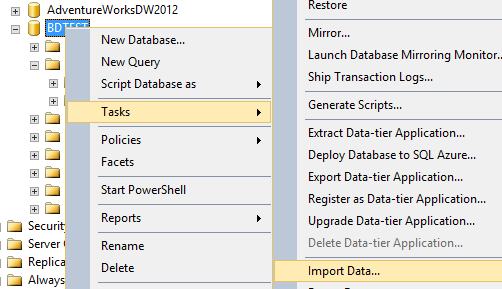
\includegraphics[width=12cm]{./Imagenes/1}
	\end{center}	

- Next y escribir el Servidor y seleccionar la base de datos

	\begin{center}
	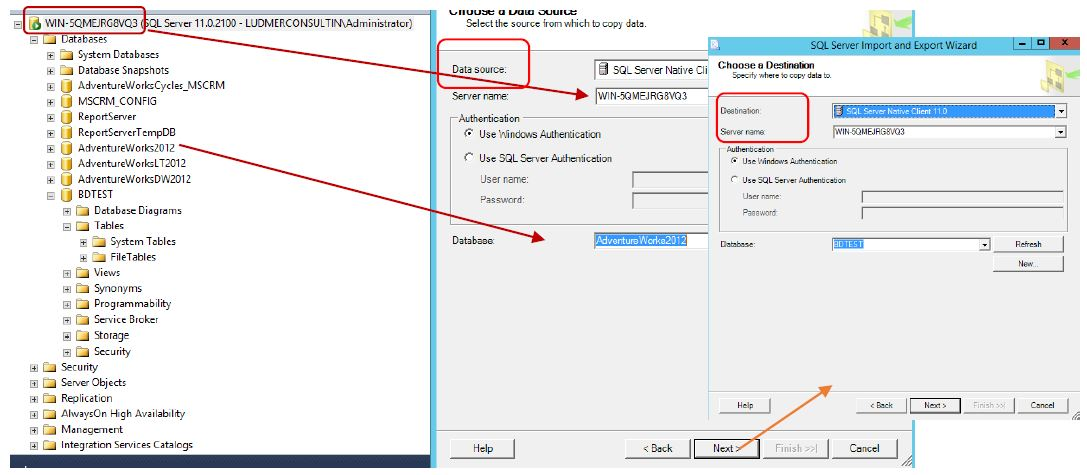
\includegraphics[width=17cm]{./Imagenes/2}
	\end{center}	

- Data Source: La base de donde vamos a importar\\
- Destination: La Base donde vamos a cargar la data

	\begin{center}
	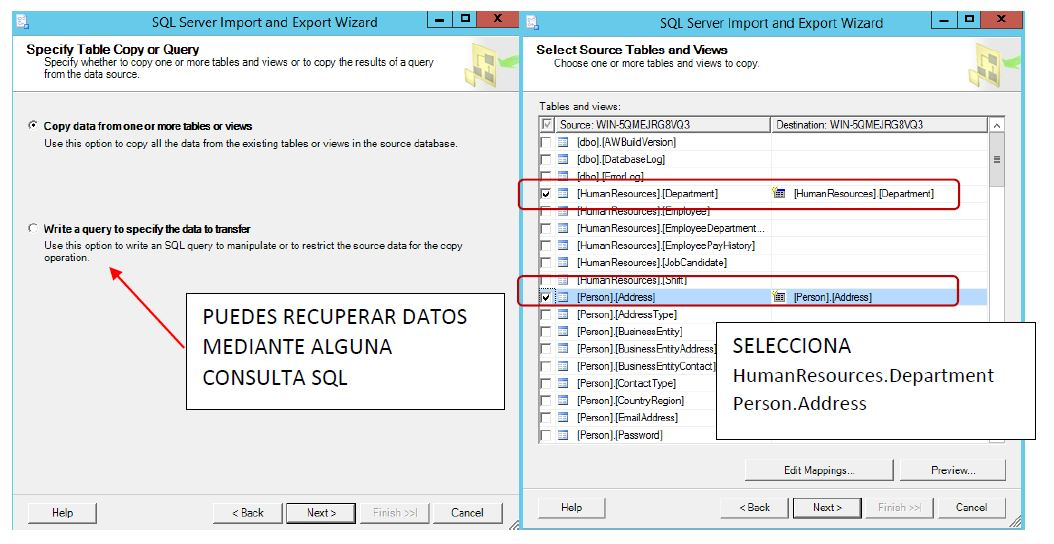
\includegraphics[width=17cm]{./Imagenes/3}
	\end{center}	

	\begin{center}
	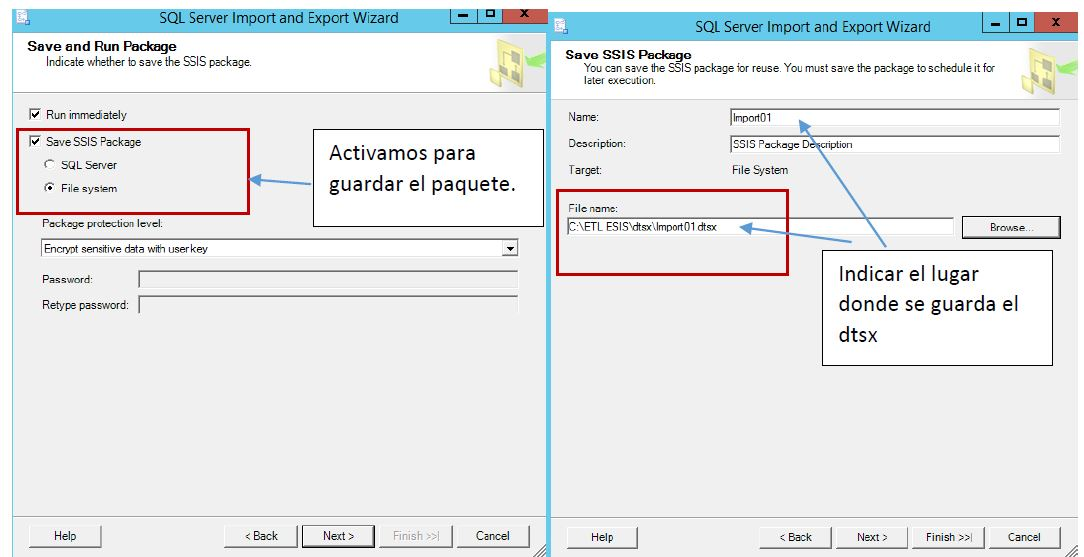
\includegraphics[width=17cm]{./Imagenes/4}
	\end{center}	

- AL Finalizar tenemos el resumen de la ejecución.\\
- HEMOS Generado nuestro 1 paquete de forma automatica.\\
- Podemos actualizar la base de datos\\
- BDTEST y encontraremos las tablas ya importadas.\\

	\begin{center}
	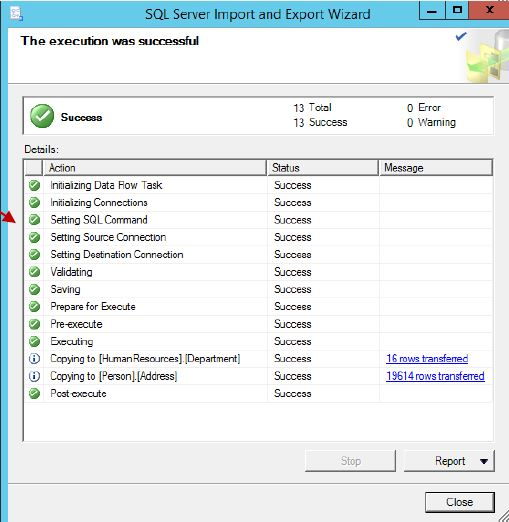
\includegraphics[width=14cm]{./Imagenes/5}
	\end{center}	

	\newpage

    \item \textbf{TAREA 2 - CREAMOS NUESTRO PRIMER PAQUETE DTSX}

	\begin{center}
	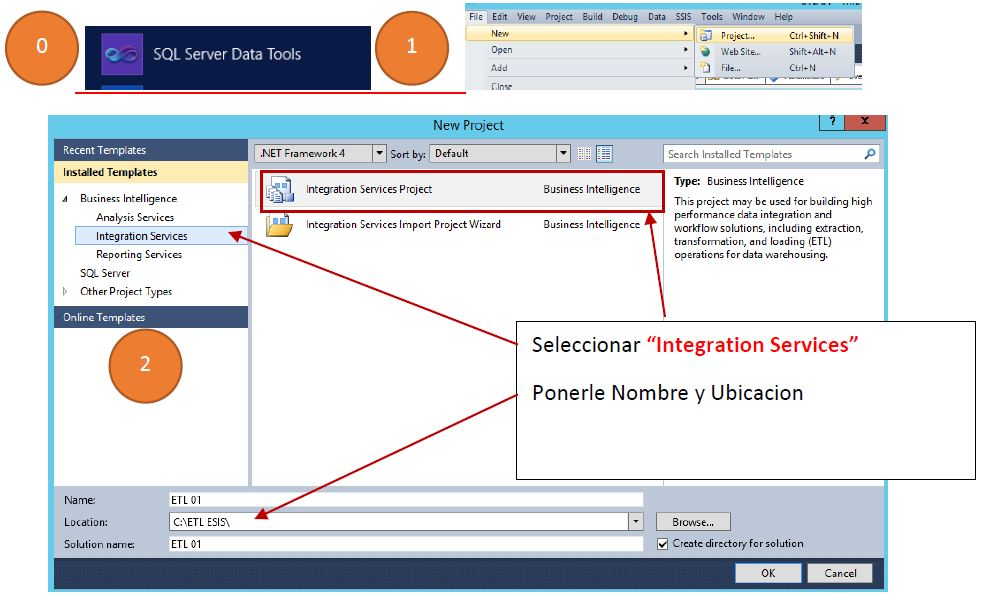
\includegraphics[width=17cm]{./Imagenes/6}
	\end{center}	

	\begin{center}
	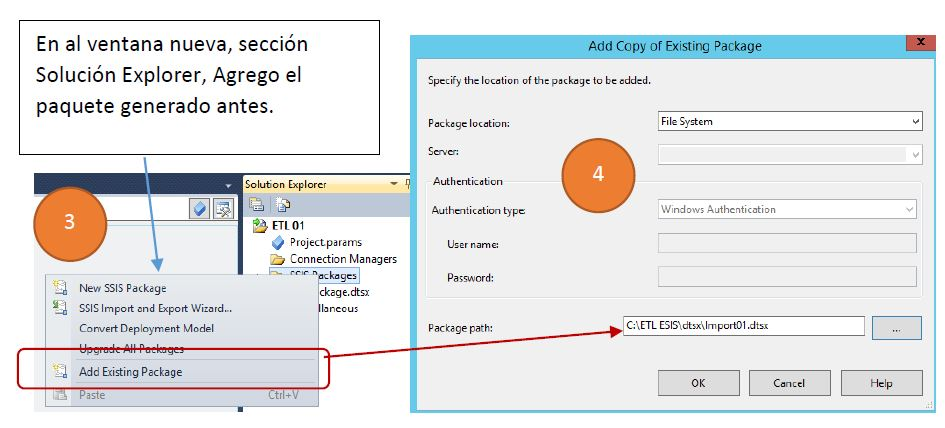
\includegraphics[width=17cm]{./Imagenes/7}
	\end{center}	

- LA SIGUIENTE VENTANA MUESTRA EL PAQUETE QUE SE HA IMPORTADO.

	\begin{center}
	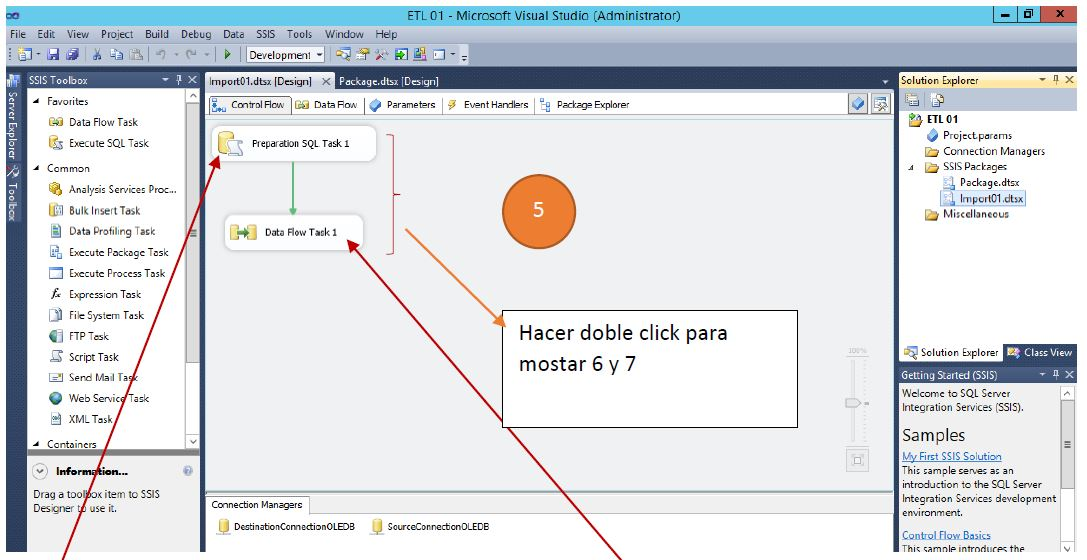
\includegraphics[width=17cm]{./Imagenes/8}
	\end{center}	

	\begin{center}
	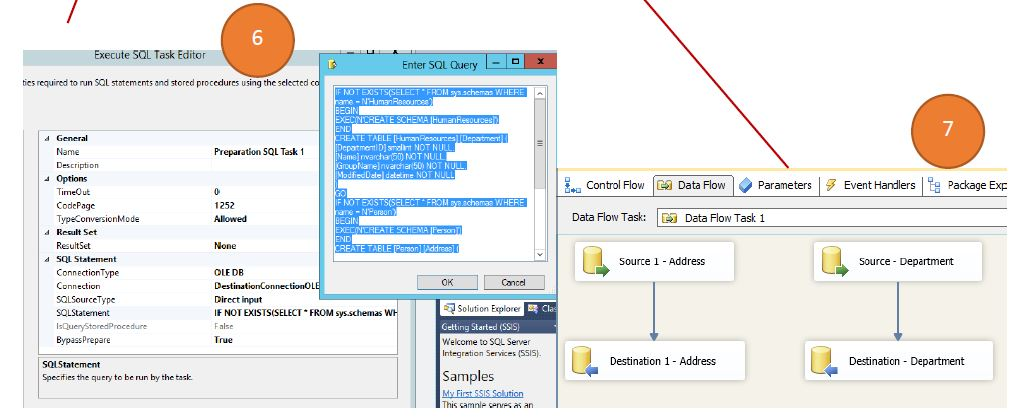
\includegraphics[width=17cm]{./Imagenes/9}
	\end{center}	
\end{itemize}